\section{Datasets}
\label{sec:datasets}

We have used datasets containing documents with a maximum word count exceeding 70,000.
We briefly discuss and analyze the word counts of the datasets below.


\subsection*{GovReport}

Introduced by \citet{huang-etal-2021-efficient}, this dataset consists of reports written
by government research agencies, including the Congressional Research Service (CRS) and
the U.S. Government Accountability Office (GAO).
Exact word count information is given in \autoref{tab:datasets}.
\autoref{fig:govreport} shows the word count distribution of the dataset.

\begin{figure}[!ht]
	\centering
	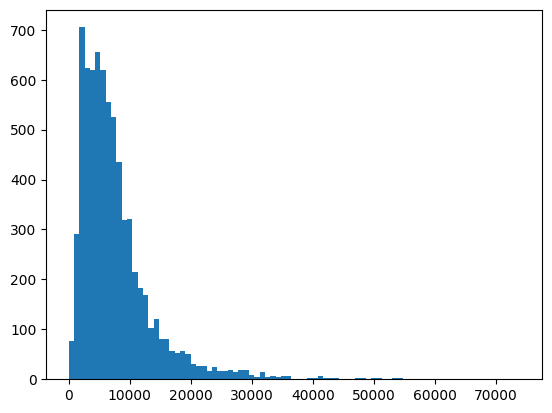
\includegraphics[width=.48\textwidth]{Images/govreport-wordcount.png}
	\caption{GovReport word counts}
	\label{fig:govreport}
\end{figure}


\subsection*{BigPatent}

Introduced in \citet{sharma-etal-2019-bigpatent}, this dataset consists of over 1.3 million
records of U.S. patent documents with human wiritten abstractive summaries.
Exact word count information is given in \autoref{tab:datasets}.
\autoref{fig:bigpatent} shows the word count distribution of the dataset.

\begin{figure}[!ht]
	\centering
	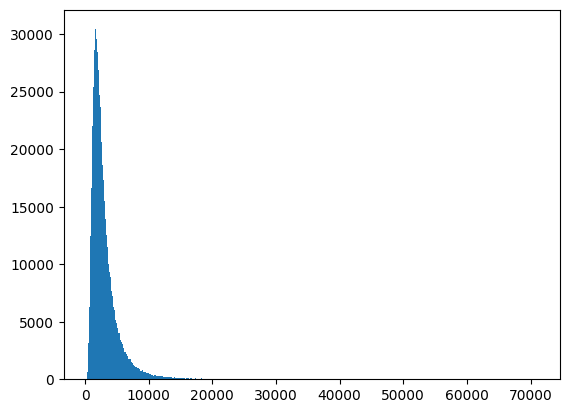
\includegraphics[width=.48\textwidth]{Images/bigpatent-wordcount.png}
	\caption{BigPatent word counts}
	\label{fig:bigpatent}
\end{figure}

\begin{table*}[!ht]
	\centering

	\begin{tabular}{c c c c}
		\hline
		Dataset & Avg. Word Count & Max Word Count & No. of Documents \\
		\hline
		GovReport & 7,700.71 & \textbf{73,815} & 7,238 \\
		BigPatent & 3,055.72 & \textbf{71,027} & 1,341,362 \\
		\hline
	\end{tabular}

	\caption{Dataset information}
	\label{tab:datasets}
\end{table*}
